%% --------------------------------------------------------------------------
% LaTeX template for the XLII CILAMCE-PANACME.
%
% This latex document tries to copy the Microsoft Word template.
% --------------------------------------------------------------------------
\documentclass[a4paper,10pt]{book}

% PACKAGES USED - packages that need to be previously installed on your computer
\usepackage[lmargin=2.5cm, rmargin=2.5cm, tmargin=2.5cm, bmargin=2.5cm ]{geometry}
\usepackage{graphicx}
\usepackage{times}
\usepackage{indentfirst}
\usepackage{fancyhdr}
\usepackage{titlesec}
\usepackage[english]{babel}
\usepackage{parskip} 
\usepackage{setspace}



%%%%%%%%%%%%%%%%%%%%%%%%%%%%%%%%%%%%%%%%%%%%%%%%%%%%%%%%%%%%%%%%%
%%%%%%%%%%%%%%%%%%%%%%%%%%%%%%%%%%%%%%%%%%%%%%%%%%%%%%%%%%%%%%%%%
%%% My Additional Packages
%%%%%%%%%%%%%%%%%%%%%%%%%%%%%%%%%%%%%%%%%%%%%%%%%%%%%%%%%%%%%%%%%
\usepackage[utf8]{inputenc}
%\usepackage{amssymb} %Mathematics
%\usepackage{amsfonts}%Mathematics
%\usepackage{amsmath,amscd}%Mathematics
%\usepackage{amsthm}%Mathematics
%\usepackage{mathrsfs}%Mathematics font
%\usepackage{xspace}
%\usepackage{booktabs}
%\usepackage{stmaryrd}%Particular Brackets
%\usepackage{graphicx} %Tables and Figures
%\usepackage{subfigure}
%\usepackage{url}
\usepackage{hyperref}
\usepackage{cleveref}
\usepackage{./pkg-crefNames}
\usepackage[labelsep=period]{caption}

%BibTeX compatible with the CILAMCE-PANACM format
\usepackage[numbers,sort&compress]{natbib}

\setlength{\bibsep}{0pt plus 0.3ex}

\renewcommand*{\bibfont}{\small}

\makeatletter
\renewcommand\bibsection
{
  \section*{References}
}



\renewenvironment{thebibliography}[1]
      {\section*{\refname}%
       \@mkboth{\MakeUppercase\refname}{\MakeUppercase\refname}%
       \list{\@biblabel{\@arabic\c@enumiv}}%
            {\settowidth\labelwidth{\@biblabel{#1}}%
             \leftmargin\labelwidth
             \advance\leftmargin-10pt% change 20 pt according to your needs
             \advance\leftmargin\labelsep
             \setlength\itemindent{10pt}% change using the inverse of the length used before
             \@openbib@code
             \usecounter{enumiv}%
             \let\p@enumiv\@empty
             \renewcommand\theenumiv{\@arabic\c@enumiv}}%
       \sloppy
       \clubpenalty4000
       \@clubpenalty \clubpenalty
       \widowpenalty4000%
       \sfcode`\.\@m}
      {\def\@noitemerr
        {\@latex@warning{Empty `thebibliography' environment}}%
       \endlist}
\renewcommand\newblock{\hskip .11em\@plus.33em\@minus.07em}
\makeatother




\makeatother
\bibliographystyle{./bib-cilamce}
%\bibliographystyle{plain}


%%%%%%%%%%%%%%%%%%%%%%%%%%%%%%%%%%%%%%%%%%%%%%%%%%%%%%%%%%%%%%%%%
%%%%%%%%%%%%%%%%%%%%%%%%%%%%%%%%%%%%%%%%%%%%%%%%%%%%%%%%%%%%%%%%%

% CONFIGURATION
\renewcommand*\arraystretch{1.5}
\renewcommand*\thesection{\arabic{section}}
%\hyphenpenalty=10000 % You can uncomment this to avoid hyphenization
\titleformat*{\section}{\large\bfseries}
\titleformat*{\subsection}{\bfseries}
\titlespacing\section{0pt}{20pt plus 2pt minus 2pt}{12pt plus 2pt minus 2pt}
\titlespacing\subsection{0pt}{20pt plus 0pt minus 0pt}{12pt plus 0pt minus 0pt}
\setlength{\parskip}{0pt} % Spacing between paragraphs
\setlength{\parindent}{0.75cm} % Paragraph identation
\setlength\abovecaptionskip{6pt}

% --------------------------------------------------------------------------
% DO NOT EDIT - SPECIAL HEADINGS OF XLI CILAMCE-PANACM
% --------------------------------------------------------------------------
\fancypagestyle{first}
{
\fancyhf{}
\fancyfoot[RO]{\footnotesize \textit{CILAMCE-PANACM 2021 \\
Proceedings of the XLII Ibero-Latin-American Congress on Computational Methods in Engineering and \\
III Pan-American Congress on Computational Mechanics, ABMEC-IACM \\
Rio de Janeiro, Brazil, November 9-12, 2021}}
\renewcommand{\headrulewidth}{.0pt}
\renewcommand{\footrulewidth}{.5pt}
}

\pagestyle{fancy}
\fancyhf{}

\fancyfoot[LE]{\footnotesize \textit{CILAMCE 2021-PANACM 2021 \\
Proceedings of the XLII Ibero-Latin-American Congress on Computational Methods in Engineering and \\
III Pan-American Congress on Computational Mechanics, ABMEC-IACM \\
Rio de Janeiro, Brazil, November 9-12, 2021}}

\fancyfoot[RO]{\footnotesize \textit{CILAMCE 2021-PANACM 2021 \\
Proceedings of the XLII Ibero-Latin-American Congress on Computational Methods in Engineering and \\
III Pan-American Congress on Computational Mechanics, ABMEC-IACM \\
Rio de Janeiro, Brazil, November 9-12, 2021}}




\renewcommand{\headrulewidth}{.5pt}
\renewcommand{\footrulewidth}{.5pt}

% --------------------------------------------------------------------------
% PLEASE, EDIT THIS!
\fancyhead[LE]{\footnotesize \textit{Template file for CILAMCE-PANACM-2021 full-length paper (enter here with the short title of your paper)}}
\fancyhead[RO]{\footnotesize \textit{G. L. L. Santos, O. B. A. Rodrigues, J. P. L. Santos}}
% --------------------------------------------------------------------------

\begin{document}\thispagestyle{first}

% --------------------------------------------------------------------------
% DO NOT EDIT - LOGO OF XLI CILAMCE
% --------------------------------------------------------------------------

\begin{figure}[ht!]
\vspace{-30pt}
\flushright
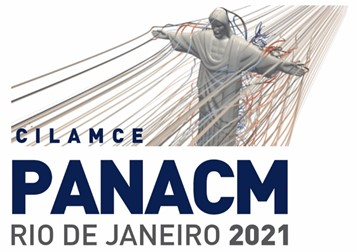
\includegraphics[width=5.5cm]{Figures/logo}
%scale=0.25
\end{figure}

% --------------------------------------------------------------------------
% TITLE OF PAPER
% --------------------------------------------------------------------------

\noindent
\textbf{\Large
Instructions for preparation and submission of full-papers for publication in the Proceedings of CILAMCE-PANACM-2021} 
\vspace{18pt} % <- keep this vertical space!

% --------------------------------------------------------------------------
% AUTHORS
% --------------------------------------------------------------------------

\noindent Gilberto L. L. Santos$^1$, Otávio B. A. Rodrigues$^1$, João P. L. Santos$^1$

\vspace{18pt} % <- keep this vertical space!


\noindent $^1$\textit{Laboratory of Scientific Computing and Visualization, Technology Center, Federal University of Alagoas \\LCCV/CTEC/UFAL}

\noindent \textit{Campus A. C. Simoes, 57072-970, Maceió/Alagoas, Brazil}

\noindent \textit{gilberto.santos@lccv.ufal.br, otavio.rodrigues@lccv.ufal.br, jpls@lccv.ufal.br}


\vspace{18pt} % <- keep this vertical space!

% --------------------------------------------------------------------------
% ABSTRACT
% --------------------------------------------------------------------------

\noindent \textbf{Abstract.}
This template file provides detailed formatting instructions for preparing your full-length paper to the Proceedings of the joint CILAMCE-PANACM-2021 (XLII Ibero-Latin American Congress on Computational Methods in Engineering and III Pan-American Congress on Computational Mechanics). It is strongly recommended that you use the pre-defined styles of this template file, as they embed all necessary text formatting for the corresponding paragraph type. Full-length papers must be written in English.

\vspace{18pt} % <- keep this vertical space!

\noindent \textbf{Keywords:} First keyword, Second keyword, Third keyword (up to 5 keywords)


% --------------------------------------------------------------------------
\section{Introduction}\label{sec:introduction}
% --------------------------------------------------------------------------
O objetivo deste trabalho é avaliar a integridade de poços com base na avaliação de sistemas de barreiras de segurança, durante as atividades de perfuração do poço. 

Com relação ao procedimento de perfuração, em poços de petróleo utilizam-se sondas de perfuração, que consistem em um conjunto de equipamentos, que podem variar quanto a sua tipologia \cite{cardoso}. A Figura \ref{fig: perf_esquema} ilustra um esquema geral da sonda na perfuração de poços. 

\begin{figure}[!ht]
\begin{center}
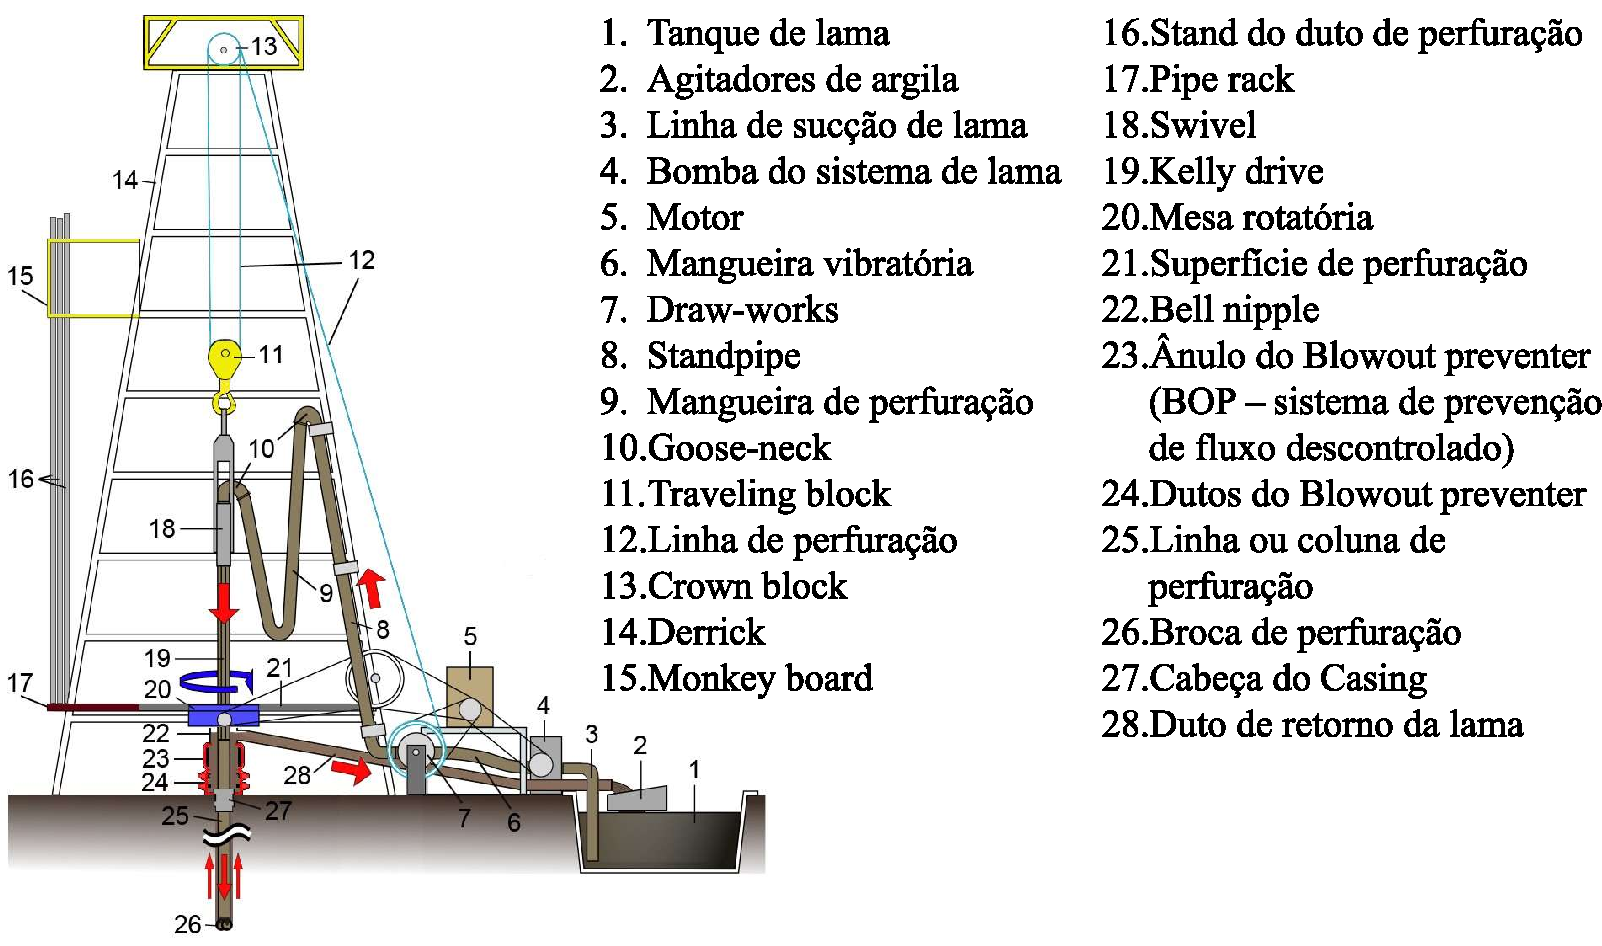
\includegraphics[scale=0.5]{Figures/perf_esquema2.pdf}
\vspace{12pt}
\caption{Esquema geral da sonda na perfuração}
\label{fig: perf_esquema}
\end{center}
\end{figure}
\vspace{8pt}
O poço é perfurado em várias fases, que são revestidas e formam as colunas de revestimento, iniciando com um tubo de pequena extensão e diâmetro maior que os posteriores. Para realizar a perfuração da fase, é necessário um conjunto de ferramentas que constitui a coluna de perfuração, tais como os tubos de perfuração e as brocas, além disso, utiliza-se o fluido de perfuração, também chamado de lama de perfuração. Estabilizar a parede da formação rochosa e carrear os cascalhos cortados pela broca são alguns dos objetivos do fluido de perfuração \cite{paranhos}.


% --------------------------------------------------------------------------
%\section{Revisão}\label{sec:revisão}%acho interessante não fazer essa seção, mas o conteúdo dela incluir na introdução
% --------------------------------------------------------------------------



% --------------------------------------------------------------------------
\section{Cenários de barreira de segurança} \label{sec:cenários}
% --------------------------------------------------------------------------



% --------------------------------------------------------------------------
\section{Resultados e discussão} \label{sec:resultados}
% --------------------------------------------------------------------------



% --------------------------------------------------------------------------
\section{Conclusão}\label{sec:Conclusão}
% --------------------------------------------------------------------------


\vspace{6pt}
\begin{center}
\begin{equation}
q_r = -4pr^2k\frac{dT}{dr}.
\label{Eq1}
\end{equation}
\end{center}
\vspace{6pt}



\vspace{8pt}
\begin{table}[!ht]
\centering
\caption{Coefficients in constitutive relations}
\label{Table1}
\vspace{0pt}
\begin{tabular}{ccc}
\hline
Constitutive relation & Nomenclature & Value \\[-2pt] \hline
Turbulent tensor & C$_{\mu}$ & 0.09 \\[-3pt]
Turbulent tensor & C$_{\mu b}$ & 0.69 \\[-3pt]
Lateral lift & C$_{L}$ & 0.08 \\[-3pt]
Virtual mass & C$_{VM}$ & 0.8 \\[-3pt] \hline
\end{tabular}
\end{table}
\vspace{8pt}


\begin{figure}[!ht]
\begin{center}
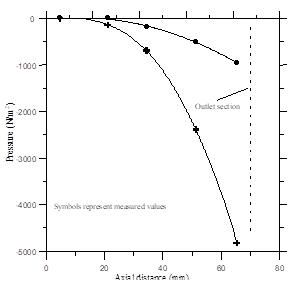
\includegraphics[scale=1.0]{Figures/Figure1.png}
\vspace{12pt}
\caption{Pressure variation along the nozzle: experimental data}
\label{Fig1}
\end{center}
\end{figure}
\vspace{8pt}


%-------------------------------------------------------------------------
\vspace{20pt}
\noindent \textbf{Acknowledgements.} This section should be positioned immediately after the Conclusion section. Type {Acknowledgements} in boldface, 10 pt Times New Roman type from left margin, leaving 20 pt line spacing before and 12pt after.
\vspace{12pt}

%--------------------------------------------------------------------------
\noindent \textbf{Authorship statement.} This section is mandatory and should be positioned immediately before the References section. The text should be exactly as follows:  The authors hereby confirm that they are the sole liable persons responsible for the authorship of this work, and that all material that has been herein included as part of the present paper is either the property (and authorship) of the authors, or has the permission of the owners to be included here. 

\bibliography{bibliography}

\end{document}
% --------------------------------------------------------------------------
